\chapterimage{orange2.jpg}
\chapterspaceabove{6.75cm} 
\chapterspacebelow{7.25cm} 
\chapter{Inequality}
throughout our mathematical journey, equalities are always the very basics of most conclusion, and that is also which we start to learn math for. However, inequalities are not such a know thing as equalities.
Inequalities have many tricky characteristics so that we have to take with care, or things could go wrong. This chapter covers the fundamentals of inequality as a crucial tool for problem-solving in Computer Science.

\section{Inequality basics}
We all know about inequalities, and the first thing to clarify is the relationship between sizes. How to determine the size relationship between certain numbers? Since the basis for comparing "numbers" with each other corresponds to one, it is stipulated on the number line that the points increase from left to right, and therefore the numbers they represent increase in turn. Listed in ascending order, that is:

Let \( a, b \) be two real numbers, and the points on the number line are denoted as \( A, B \) respectively. If \( A \) is to the right of \( B \), we say \( a > b \); if \( A \) is to the left of \( B \), we say \( a < b \); if \( A \) coincides with \( B \), we say \( a = b \).

Thus, for any two real numbers, one and only one of the following three situations must hold:

\[
a > b; \quad a = b; \quad a < b.
\]

The above relationship is also known as the one-dimensional coordinate law.

\[
\begin{aligned}
a > b &\Leftrightarrow a - b > 0 \\
a < b &\Leftrightarrow a - b < 0 \\
a = b &\Leftrightarrow a - b = 0
\end{aligned}
\]

Where the symbol “\( \Leftrightarrow \)” (double arrow), read as "if and only if," means that the truth of two propositions depends on each other. That is to say, if one proposition is true, then the other proposition is also true; conversely, if one proposition is false, then the other proposition is also false.

Based on the derivation of inequalities, in most cases, the above principles are sufficient. The following mathematical laws involve the geometric and algebraic meanings of the sizes of real numbers and the relationship between them. They are the basis for comparing the sizes of two real numbers and for proving inequalities by comparison. Let's review some basic properties of inequalities that are the foundation for our further study.

\begin{itemize}
    \item Symmetry: \( a > b \) if and only if \( b < a \).
    \item Transitivity: If \( a > b \) and \( b > c \), then \( a > c \).
    \item Addition (Subtraction): If \( a > b \), then \( a + c > b + c \).
    \item Multiplication (Division): If \( a > b \) and \( c > 0 \), then \( ac > bc \); if \( a > b \) and \( c < 0 \), then \( ac < bc \).
    \item Exponentiation: If \( a > b \), then \( a^n > b^n \), where \( n \) is a positive integer, and \( n \geq 2 \).
    \item Root Extraction (Power Root): If \( a > b > 0 \), then \( \sqrt[n]{a} > \sqrt[n]{b} \), where \( n \) is a positive integer, and \( n \geq 2 \).
    \item If \( a > b \) and \( c > d \), then \( a + c > b + d \).
    \item If \( a > b > 0 \) and \( c > d > 0 \), then \( ac > bd \).
\end{itemize}
\subsection{Exercises}
\begin{exercise}
    Explain the following statement.
    \begin{enumerate}
        \item If \( a > b \), then \( \frac{a}{c} > \frac{b}{c} \);
        \item If \( ac < bc \), then \( a < b \);
        \item If \( a < b \), then \( \frac{1}{a} > \frac{1}{b} \);
        \item If \( ac^2 > bc^2 \), then \( a > b \);
        \item If \( a > b \), then \( a^n > b^n \).
    \end{enumerate}
\end{exercise}

\textbf{Solution:}

\begin{enumerate}
    \item If \( c > 0 \), multiplying both sides of \( a > b \) by the positive number \( \frac{1}{c} \) preserves the inequality, hence \( \frac{a}{c} > \frac{b}{c} \). If \( c < 0 \), the direction of the inequality would be reversed, which is not given in the condition, hence we assume \( c > 0 \).
    \item Dividing both sides of \( ac < bc \) by \( c \) (assuming \( c \neq 0 \)), we get \( a < b \) because division by a positive number preserves the inequality, and division by a negative number reverses it.
    \item Taking the reciprocal of both sides of \( a < b \) reverses the inequality because \( a \) and \( b \) are on opposite sides of the fraction line, hence \( \frac{1}{a} > \frac{1}{b} \) (assuming \( a, b > 0 \) to avoid division by zero).
    \item Dividing both sides of \( ac^2 > bc^2 \) by \( c^2 \) (assuming \( c \neq 0 \)) preserves the inequality, hence \( a > b \) because \( c^2 \) is positive regardless of whether \( c \) is positive or negative.
    \item Raising both sides of \( a > b \) to a power \( n \) (assuming \( n \) is a positive integer) preserves the inequality because both \( a \) and \( b \) are raised to the same power, hence \( a^n > b^n \).
\end{enumerate}
\begin{exercise}
    Given the inequality \( a > b > 0 \), \( c < d < 0 \), \( f < 0 \), show that:
\[
\frac{f}{a - c} > \frac{f}{b - d}.
\]
\end{exercise}
\begin{proof}
    Since \( a > b > 0 \) and \( c < d < 0 \), then \( a - c > b - d \) because subtracting a smaller negative number is the same as adding a larger positive number. Given that \( f < 0 \), when dividing by a larger positive number, the result is smaller because a negative number divided by a positive number yields a negative result, and the further away the divisor is from zero, the smaller the quotient.

Therefore:
\[
\frac{f}{a - c} > \frac{f}{b - d}.
\]
\end{proof}

\section{Solving Quadratic Inequality}
Recall that, when we solve Quadratic equations, we use discriminant to solve equations, which is also applicable to inequalities.
For a quadratic inequality of the form $ax^2 + bx + c > 0$ or $ax^2 + bx + c < 0$ (where $a > 0$), the solution set can be determined by the discriminant $\Delta = b^2 - 4ac$:
\begin{enumerate}
    \item If $\Delta > 0$, the quadratic equation $ax^2 + bx + c = 0$ has two distinct real roots $x_1$ and $x_2$, and $x_1 < x_2$. The solution set for $y = ax^2 + bx + c$ being greater than zero (when $y = 0$) is for values of $x$ either less than $x_1$ or greater than $x_2$, and the solution set for $ax^2 + bx + c < 0$ is $\{ x \mid x_1 < x < x_2 \}$.
    \item If $\Delta = 0$, then $ax^2 + bx + c = 0$ has one real root, specifically $x_1 = x_2 = -\frac{b}{2a}$. The solution set for $y = ax^2 + bx + c$ being greater than zero is all $x$ except $x \neq -\frac{b}{2a}$, and there is no solution set where $ax^2 + bx + c < 0$.
    \item If $\Delta < 0$, then $ax^2 + bx + c = 0$ has no real roots, and the parabola $y = ax^2 + bx + c$ does not intersect the x-axis. The solution set for $ax^2 + bx + c > 0$ is all real numbers, and there is no solution set where $ax^2 + bx + c < 0$.
\end{enumerate}
\begin{figure}[ht!]
    \centering
    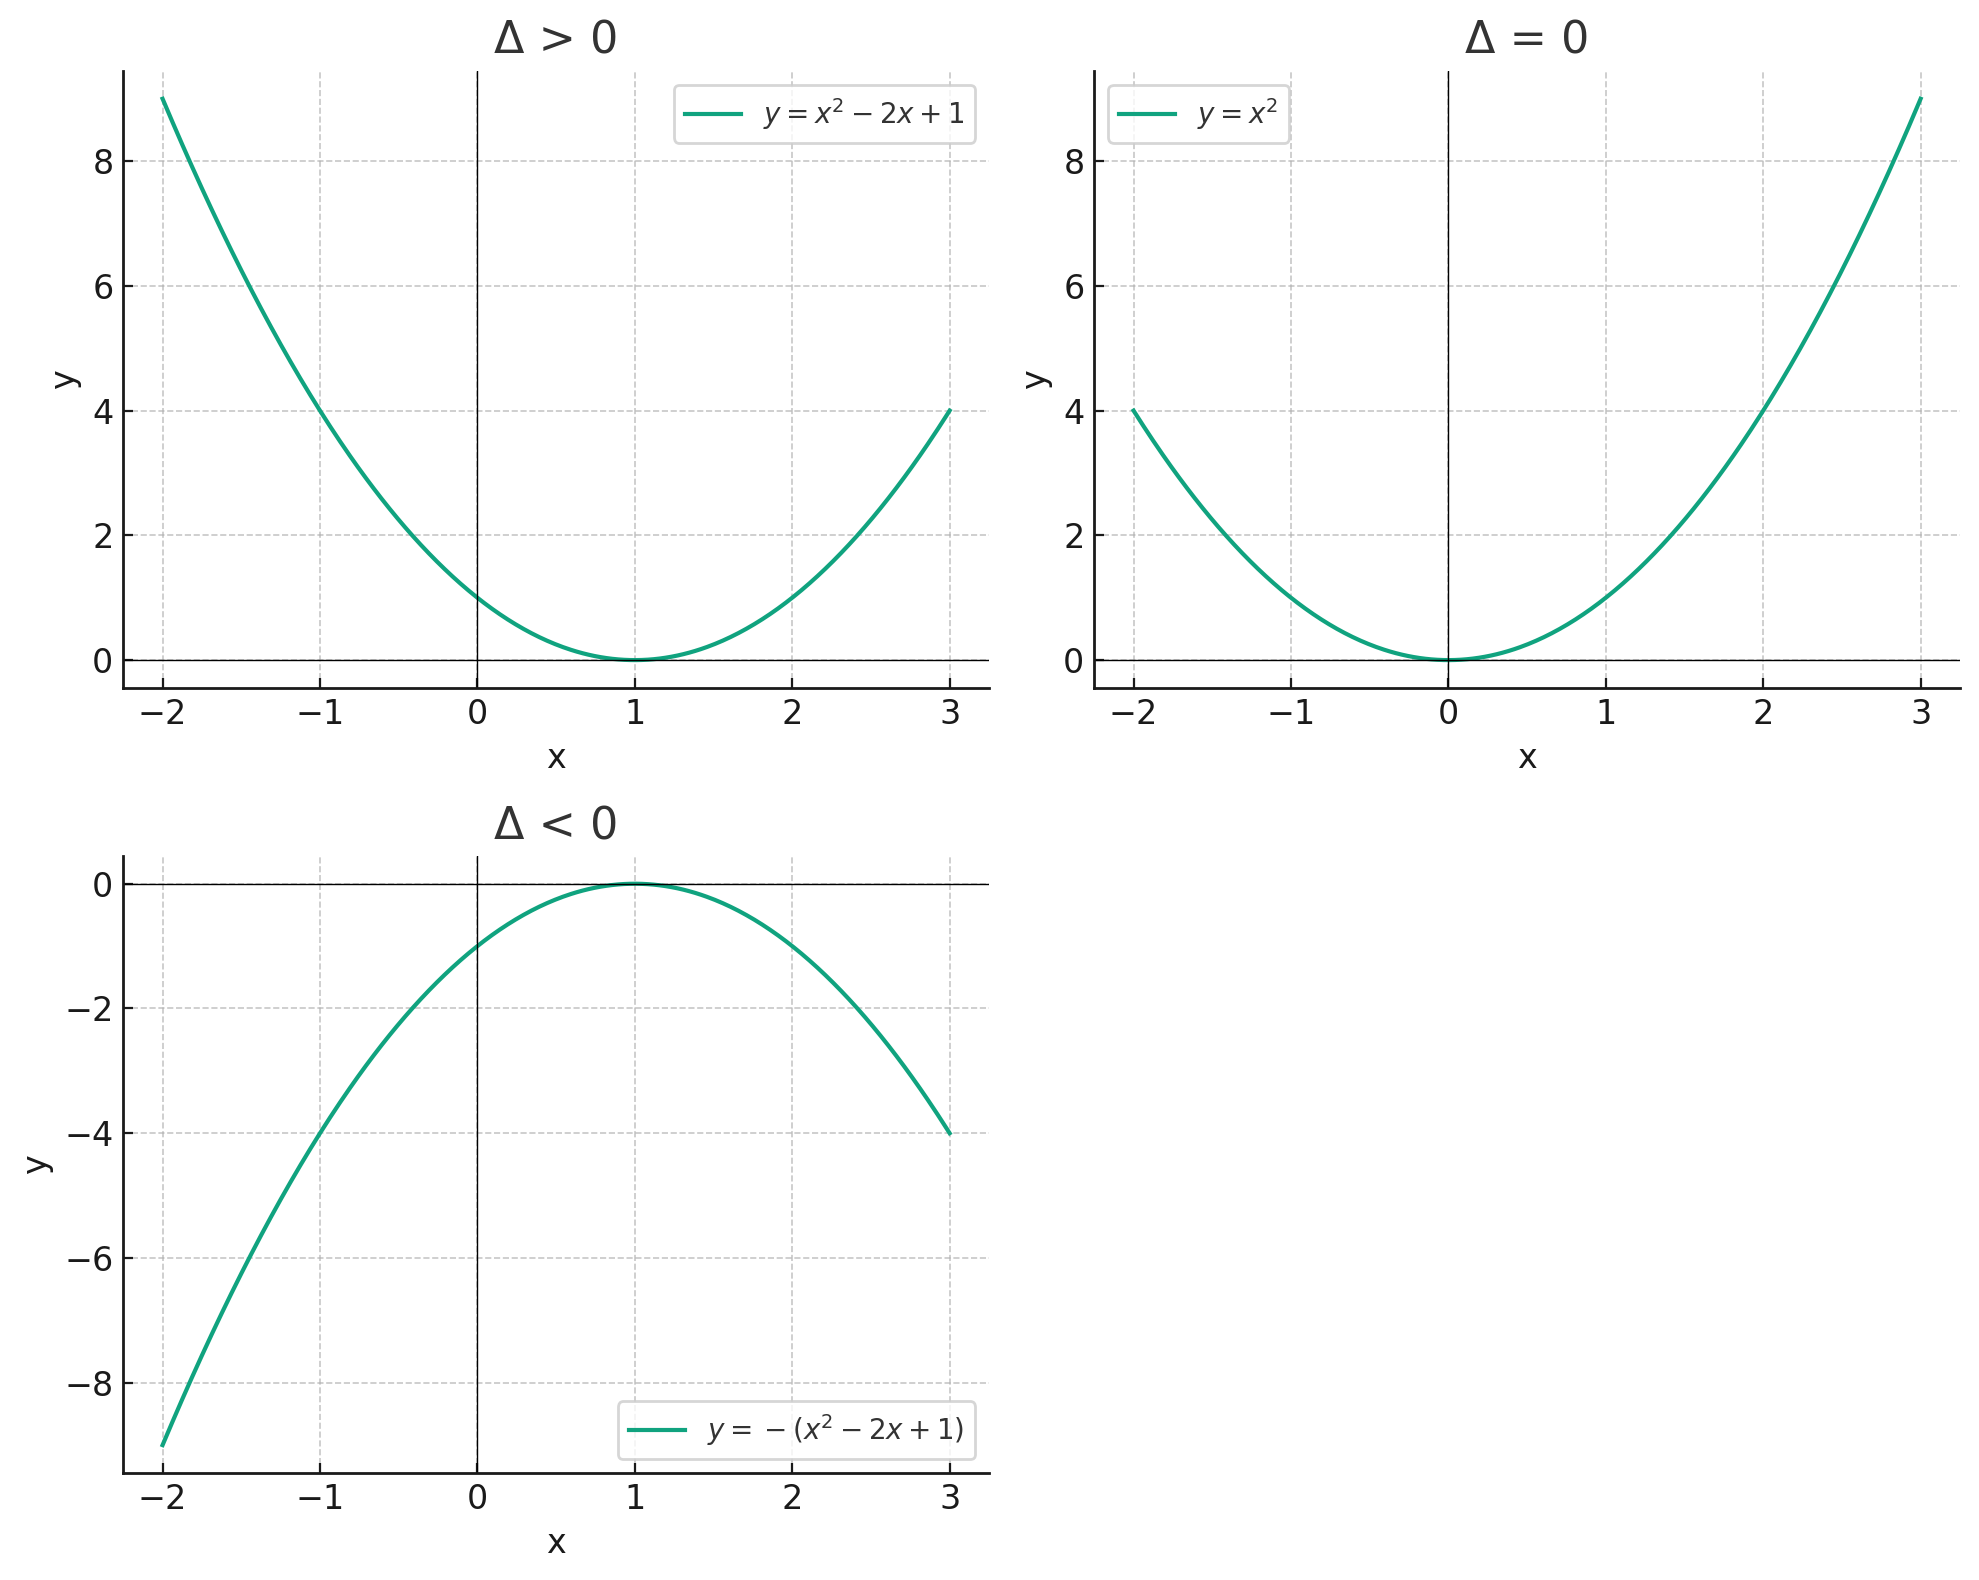
\includegraphics[width=0.8\textwidth]{quadratic.png}
    \caption{Quadratic function graphs based on the discriminant.}
\end{figure}